% PLANTILLA APA7
% Creado por: Isaac Palma Medina
% Última actualización: 25/07/2021
% @COPYLEFT

% Fuentes consultadas (todos los derechos reservados):  
% Normas APA. (2019). Guía Normas APA. https://normas-apa.org/wp-content/uploads/Guia-Normas-APA-7ma-edicion.pdf
% Tecnológico de Costa Rica [Richmond]. (2020, 16 abril). LaTeX desde cero con Overleaf (1 de 3) [Vídeo]. YouTube. https://www.youtube.com/watch?v=kM1KvHVuaTY Weiss, D. (2021). 
% Formatting documents in APA style (7th Edition) with the apa7 LATEX class. https://ctan.math.washington.edu/tex-archive/macros/latex/contrib/apa7/apa7.pdf @COPYLEFT

%+-+-+-+-++-+-+-+-+-+-+-+-+-++-+-+-+-+-+-+-+-+-+-+-+-+-+-+-+-+-++-+-+-+-+-+-+-+-+-+

% Preámbulo
\documentclass[stu, 12pt, letterpaper, donotrepeattitle, floatsintext, natbib, helv]{apa7}
\usepackage{listings}
\usepackage[utf8]{inputenc}
\usepackage{comment}
\usepackage{marvosym}
\usepackage{graphicx}
\usepackage{float}
\usepackage[normalem]{ulem}
\usepackage[spanish]{babel} 
%\usepackage{titling}
\let\apasubparagraph\subparagraph
\let\subparagraph\paragraph
\usepackage[compact]{titlesec}
\let\subparagraph\apasubparagraph
\usepackage{hyperref}
\selectlanguage{spanish}
\useunder{\uline}{\ul}{}
\newcommand{\myparagraph}[1]{\paragraph{#1}\mbox{}\\}
\graphicspath{{./Images/}}
\titleformat{\section}{\normalfont\large\bfseries}{\thetitle. \quad }{0pt}{}[{ \titlerule[0.8pt]}]
\titleformat{\subsection}{\normalfont\bfseries}{}{}{}[]

% Portada

\begin{document}
\begin{titlepage}
    \centering
    \vfill
    \LARGE Análisis de métodos de buscar\\
    \vskip2cm
    \large Diego Quirós Artiñano \\
    Universidad Nacional de Costa Rica \\
    EIF-203: Estructuras Discretas (10 A.M.) \\ 
    Carlos Loria-Saenz \\
    24 de marzo, 2022 \\
    \vfill
    
\includegraphics[width = 0.4\textwidth]{/home/xarthy/UNAImage/UNA.png} \\
    \vfill
    \vfill
    % (autores separados, consultar al docente)
    % Manera oficial de colocar los autores:
    %\author{Autor(a) I, Autor(a) II, Autor(a) III, Autor(a) X}
\end{titlepage}

% Índices
\pagenumbering{roman}
    % Contenido
\renewcommand\contentsname{\largeÍndice}
\tableofcontents
\setcounter{tocdepth}{2}
\newpage
    % Figuras
\renewcommand{\listfigurename}{\largeÍndice de fíguras}
\listoffigures
\newpage
    % Tablas
\renewcommand{\listtablename}{\largeÍndice de tablas}
\listoftables
\newpage

% Cuerpo
\pagenumbering{arabic}

%------------------------------------------------------------------------------------
\section{Análisis de es\_simetrica()}
\begin{enumerate}
    \setcounter{enumi}{-1}
    \item El algoritmo original.
\end{enumerate}
\begin{lstlisting}[language=Python]
    def es_simetrica(a:list[list[int]])-> bool:
        for i in range(len(a)):
            for j in range(i+1, len(a[i])):
                if i != j and a[i][j] != a[j][i]:
                    return False
        return True
\end{lstlisting}
\begin{enumerate}
    \setcounter{enumi}{0}
    \item Tamaño de los datos \\s
El método se construyó de manera en la que no busque la diagonal de la matriz y solo se tiene que buscar la parte de arriba, entonces el tamaño de datos es $\frac{n(n-1)}{2}$
    \item Operaciones de Interés \\
    \begin{table}[h]
        \centering
        \begin{tabular}{|c c c|} 
         \hline
         Notación [en función de tiempo (T)] & Operación & Tipo de Operación \\ [0.5ex] 
         \hline\hline
         $T_{range()}$ & range(len(a)) or range(i+1, len(a[i])) & constante \\ 
         \hline
         $T_{!=}$ & i != j or a[i][j] != a[j][i] & constante \\
         \hline
         $T_{[]}$ & a[i][j] or a[j][i] & constante \\ [1ex]
         \hline
        \end{tabular}
        \caption{Operaciones es\_simetrica()}
        \label{tab:tablesimetrica}
    \end{table}
        Peor caso: toas son iguales a la mas grande de todas, como supuesto \\
        Asumimos que vale 1 (unidad de tiempo), según el más alto
    \item Ecuación
    \end{enumerate}
\begin{lstlisting}[language=Python]
    # Separando por partes
    # Parte 1
    for i in range(len(a)):
        # Parte 2.1
        for j in range(i+1, len(a[i])):
            Parte 2.2
            if i != j and a[i][j] != a[j][i]:
                return False
    # Parte 3
    return True
\end{lstlisting}

\[T_{es\_simetrica()}(n) = T_{parte1} + T_{parte2} + T_{parte3} \] \\ 
\[T_{es_simetrica()}(n) = 1 + T_{for()}(n) + 0\] \\
\[T_{es_simetrica()}(n) = T_{for()}(n) + 1\] \\
Evaluando $T_{for()}(n)$: (Parte 2.1) \\
1 operación: del range cada vez que i cambia \\

Entonces: \[T_{for()}(n) = 1 + T_{for()_{for()}} + T_{for()}(n-1)\] \\
\[T_{for()}(n) = 1 + T_{for()_{for()}}(n) + 1 + T_{for()_{for()}}(n-1) + 1 + T_{for()_{for()}}(n-2) + ... T_{for()}(0)\] \\
\[T_{for()}(n) = n + T_{for()_{for()}}(n) + T_{for()_{for()}}(n-1) + ... T_{for()_{for()}}(1)\] \\

Evaluando para $T_{for()_{for()}}(n)$: (2.2)
6 operaciones: != y los 4 $[]$'s cada vez que cambia j\\
\[T_{for()_{for()}}(n) = 2 + 4 + T_{for()_{for()}}(n-1)\] \\ 
\[T_{for()_{for()}}(n) = 6 + 6 + 6 + ... + T_{for()_{for()}}(0)\] \\
$T_{for()_{for()}}(0)$ es igual a 0 porque sale del for sin verificar otra vez
\[T_{for()_{for()}}(n) = 6n\]
Metiendolo en la Parte 2.1
\[T_{for()}(n) = n + 6n + 6(n-1) + 6(n-2) + ... + 6\] \\ 
\[T_{for()}(n) = n + 6(\frac{n*(n+1)}{2})\] \\


\begin{enumerate}
    \setcounter{enumi}{3}
    \item Volviendo a meter en la ecuación original:
    \[T_{es_simetrica()}(n) = n + 6(\frac{n*(n+1)}{2}) + 1\] \\
    \[T_{es_simetrica()}(n) = (n + 1) + 6(\frac{n*(n+1)}{2})\] \\
    \[T_{es_simetrica()}(n) = (n + 1) + 3(n*(n + 1))\] \\
    \[T_{es_simetrica()}(n) = (n + 1) + 3(n^2 + n)\] \\
    \[T_{es_simetrica()}(n) = 3n^2 + 4n + 1\] \\
    \item Orden de crecimiento \\
El orden de crecimiento es el que es cuando la ecuación de tiempo es parabólica.
    \item Código
\end{enumerate}
\begin{lstlisting}[language=Python]
    def es_simetrica_instrumentado(a:'list[list[int]]')-> int:
        contador_operaciones:int = 0
        contador_operaciones += 1 # range de afuera
        for i in range(len(a)):
            contador_operaciones += 1 # cada range nuevo cuando cambia el i
            for j in range(i, len(a[i])):
                contador_operaciones += 6 # 2 != y 4 []'s
                if i != j and a[i][j] != a[j][i]:
                    return contador_operaciones
        return contador_operaciones
\end{lstlisting}

\section{Excel}
Para importar a Excel para hacer la gráfica, se hizo este código:
{\scriptsize
\begin{lstlisting}[language=Python]
    def test_simetrica_instrumentado(filename, init, maxi, inc):
        file = open(filename, 'w')
        file.write('n;time\n')
        for n in range(init, maxi, inc):
            a = []
            for i in range(n):
                a.append([])
                for j in range(n):
                    a[i].append(1)
            file.write(f'{n};{es_simetrica_instrumentado(a)}\n')
        file.close()
    test_simetrica_instrumentado('simetrica_instrumentado.csv', 10, 200, 10)
\end{lstlisting}}

\begin{figure}[h]
    \centering
    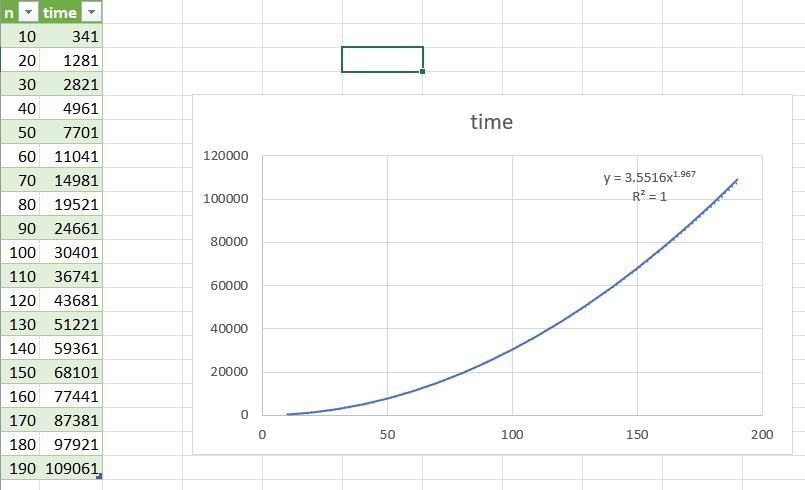
\includegraphics[width=1\textwidth]{Screenshot 2022-03-24 044713.png}
    \caption{Gráfica del método en Excel}
    \label{fig:figureExcel1}
\end{figure}
\nocite{Clase21Mar}
\newpage
\renewcommand\refname{\large\textbf{Referencias}}
\bibliography{ref}

\end{document}